\section{Pruebas}
\label{sec:pruebas}

En esta sección se describen los escenarios de prueba, cómo ejecutarlos y cómo interpretar los resultados. El objetivo es validar que el sistema cumple con los requisitos de rendimiento y escalabilidad definidos en la sección \ref{sec:atributos-importantes}.

\subsubsection{Correr los escenarios}

Todos los comandos se ejecutan desde el directorio \texttt{perf/}.

\begin{verbatim}
cd perf
\end{verbatim}

\paragraph{Escenarios disponibles}

\begin{table}[H]
\centering
\begin{tabular}{lll}
\toprule
\textbf{Archivo} & \textbf{Endpoint principal} & \textbf{Uso} \\
\midrule
\texttt{rates.yaml} & GET /rates & Solo lectura, mínima lógica \\
\texttt{exchange.yaml} & POST /exchange & Operación crítica con lógica de negocio \\
\texttt{mixed.yaml} & Mix 60/30/5/5 & Perfil de tráfico realista \\
\bottomrule
\end{tabular}
\end{table}

\paragraph{Workloads disponibles}

\begin{table}[H]
\centering
\setlength{\tabcolsep}{8pt}
\begin{tabular}{lllp{5cm}}
\toprule
\textbf{Workload} & \textbf{Duración aprox.} & \textbf{Carga} & \textbf{Pregunta que responde} \\
\midrule
\texttt{baseline} & 3 min & 1 req/s constante & ¿Funciona sin errores con mínima carga? \\
\texttt{load} & 7 min & Ramp 1→20, luego 20 req/s & ¿Cómo se comporta bajo carga normal? \\
\texttt{stress} & 10 min & Escalado 10→25→50→100 rps & ¿En qué punto aparecen errores o degradación? \\
\bottomrule
\end{tabular}
\end{table}

\subsubsection{Comandos}

\begin{verbatim}
# Siempre empezar con baseline para verificar que todo funciona
./run-scenario.sh rates baseline
./run-scenario.sh exchange baseline
./run-scenario.sh mixed baseline

# Load test (el más relevante para comparar antes/después de mejoras)
./run-scenario.sh rates load
./run-scenario.sh exchange load
./run-scenario.sh mixed load

# Stress test (para encontrar el punto de quiebre)
./run-scenario.sh exchange stress
./run-scenario.sh mixed stress
\end{verbatim}

\begin{quote}
\textbf{Nota:} Los resultados JSON se guardan automáticamente en \texttt{perf/results/} con timestamp.
\end{quote}

Para \texttt{rates.yaml} (tiene solo el environment \texttt{api}):

\begin{verbatim}
npm run api
# o
npm run artillery -- run rates.yaml -e api
\end{verbatim}

\subsubsection{Leer los resultados en tiempo real (Grafana)}

Mientras corre Artillery, abrir el dashboard en \texttt{http://localhost:80}:

\begin{itemize}[leftmargin=*]
    \item \textbf{Scenarios launched} → cuántos requests/s está enviando Artillery.
    \item \textbf{Requests state} → proporción de 200 OK vs 5xx. Si los 5xx aumentan, el sistema está degradado.
    \item \textbf{Response time} → observar la línea \texttt{p95} y \texttt{p99}. Si se separan de la mediana, hay cola larga.
    \item \textbf{Resources} → CPU\% y memoria\% del contenedor seleccionado. Cambiar el selector \texttt{\$container} para ver cada instancia (\texttt{exchange-api-1}, \texttt{exchange-api-2}, \texttt{exchange-api-3}).
\end{itemize}

\textbf{Tip:} Ajustar el rango de tiempo del dashboard a ``Last 5 minutes'' o ``Last 15 minutes'' para que los datos sean visibles durante la prueba.

\subsubsection{Generar reporte HTML (post-prueba)}

Después de cada escenario, el script indica el comando exacto. En general:

\begin{verbatim}
npx artillery report -o results/mi-reporte.html results/exchange-load-20260504-123456.json
\end{verbatim}

Abrir el HTML en el browser para ver latencias, errores y distribución de respuestas con gráficos.

\subsubsection{Guardar evidencia para el informe}

Para cada escenario ejecutado, guardar:
\begin{enumerate}[leftmargin=*]
    \item El archivo \texttt{.json} de resultados en \texttt{perf/results/} (ya se guarda automáticamente).
    \item Un screenshot del dashboard de Grafana al finalizar la prueba (especialmente los paneles de \textit{Response time} y \textit{Requests state}).
\end{enumerate}


\subsection{Objetivo}

Obtener un panorama cuantitativo y reproducible del comportamiento del servicio bajo distintos regímenes de carga. Las mediciones deben permitir:

\begin{enumerate}[leftmargin=*]
    \item Establecer un \textbf{baseline} del estado actual del sistema antes de aplicar cualquier mejora.
    \item Identificar los \textbf{puntos de ruptura} (saturación, degradación, crash).
    \item Proveer la \textbf{línea de comparación} contra la cual medir el impacto de las tácticas que se implementen en etapas posteriores (caching, locking, Redis, réplicas, etc.).
    \item Correlacionar métricas de cliente (Artillery), de contenedor (cAdvisor) y de aplicación (instrumentación a agregar) en un único dashboard.
\end{enumerate}

\subsection{Estado Actual de la Infraestructura de Carga y Métricas}

\subsubsection{Lo que ya está armado}

\begin{table}[H]
\centering
\begin{tabular}{lp{4cm}p{4cm}}
\toprule
\textbf{Componente} & \textbf{Archivo / Ubicación} & \textbf{Estado} \\
\midrule
Artillery con plugin StatsD & \texttt{perf/rates.yaml}, \texttt{perf/package.json} & Funcional, solo cubre \texttt{GET /rates} \\
Script de ejecución & \texttt{perf/run-scenario.sh} & Wrapper para correr escenarios \\
StatsD + Graphite & \texttt{docker-compose.yml} (graphite), \texttt{statsd.config.json}, \texttt{graphite.storage-schemas.conf} & Corriendo, retención de 6 h @ 10 s \\
cAdvisor & \texttt{docker-compose.yml} (cadvisor) & Corriendo, envía a StatsD con prefijo \texttt{cadvisor} \\
Grafana dashboard & \texttt{perf/dashboard.json} & 4 paneles: RPS, códigos HTTP, latencia cliente, CPU/memoria \\
\bottomrule
\end{tabular}
\end{table}

\subsubsection{Lo que falta}

\begin{itemize}[leftmargin=*]
    \item \textbf{Escenarios de carga para los endpoints críticos} (\texttt{POST /exchange}, \texttt{PUT /rates}, carga mixta). El único escenario actual es \texttt{GET /rates}, que no ejercita la lógica de negocio real.
    \item \textbf{Instrumentación de la aplicación}: la app no emite ninguna métrica propia a StatsD.
    \item \textbf{Endpoint de healthcheck} (\texttt{/health}), necesario para healthcheck de Docker y para correlacionar disponibilidad con métricas.
    \item \textbf{Panel de Grafana con métricas de negocio y percentiles p95/p99} (el panel actual solo muestra mediana y máximo).
    \item \textbf{Anotaciones de Grafana} marcando inicio/fin de cada escenario de prueba para correlación visual.
\end{itemize}

\subsection{Workload Models (Modelos de Carga)}

Basado en Artillery Workload Models y la distinción load vs stress testing de los artículos provistos, se proponen 5 modelos diferenciados. Cada uno responde a una pregunta distinta.

\subsubsection{Baseline (Smoke / Low-Constant)}

\textbf{Pregunta:} ¿Cuál es el comportamiento del sistema bajo carga mínima, sin estrés?

\begin{itemize}[leftmargin=*]
    \item \textbf{Duración:} 3 minutos.
    \item \textbf{Carga:} 1 req/s constante.
    \item \textbf{Propósito:} Medir latencia base, verificar que no hay errores en condiciones ideales. Usado como referencia para comparar con cargas mayores.
\end{itemize}

\subsubsection{Load Test (Carga Normal Sostenida)}

\textbf{Pregunta:} ¿Cómo se comporta el sistema bajo la carga esperada en producción?

\begin{itemize}[leftmargin=*]
    \item \textbf{Duración:} 10 minutos.
    \item \textbf{Carga:} Ramp 1$\rightarrow$20 req/s en 2 min, constante 20 req/s durante 8 min.
    \item \textbf{Propósito:} Observar comportamiento estable bajo carga esperada. Los problemas deben manifestarse como latencia elevada o tasa de error creciente.
\end{itemize}

\subsubsection{Stress Test (Buscar el Punto de Quiebre)}

\textbf{Pregunta:} ¿Cuál es la capacidad máxima del sistema antes de degradarse?

\begin{itemize}[leftmargin=*]
    \item \textbf{Duración:} 15 minutos.
    \item \textbf{Carga:} Ramp 1$\rightarrow$200 req/s escalonado (10, 25, 50, 100, 200 req/s, 3 min en cada escalón).
    \item \textbf{Propósito:} Identificar el knee point de la curva de latencia y el RPS al que aparecen los primeros errores. Exhibe la race condition de \texttt{exchange()}.
\end{itemize}

\subsubsection{Spike Test}

\textbf{Pregunta:} ¿Cómo responde el sistema a un pico repentino de tráfico?

\begin{itemize}[leftmargin=*]
    \item \textbf{Duración:} 5 minutos.
    \item \textbf{Carga:} 2 req/s durante 1 min $\rightarrow$ salto instantáneo a 100 req/s durante 30 s $\rightarrow$ vuelta a 2 req/s durante el resto.
    \item \textbf{Propósito:} Observar la recuperación tras saturación. Con una sola instancia y sin rate limiting, se espera que el spike sature el event loop y la latencia tarde en volver al baseline incluso después de que la carga disminuya.
\end{itemize}

\subsubsection{Soak / Endurance Test}

\textbf{Pregunta:} ¿El sistema degrada con el tiempo bajo carga moderada?

\begin{itemize}[leftmargin=*]
    \item \textbf{Duración:} 60 minutos.
    \item \textbf{Carga:} 10 req/s constante.
    \item \textbf{Propósito:} Exhibir el memory leak del \texttt{log} y la degradación del \texttt{scheduleSave} al crecer el array. Espera observable: CPU y memoria crecientes, latencia creciente, eventualmente crash por OOM si se corre suficiente tiempo.
\end{itemize}

\subsection{Escenarios de Artillery a Implementar}

Cada uno de los 5 workload models se ejecutará sobre cada uno de los siguientes escenarios para aislar el comportamiento por tipo de operación.

\subsubsection{\texttt{perf/rates.yaml} (ya existe)}

\begin{itemize}[leftmargin=*]
    \item \textbf{Target:} \texttt{GET /rates}
    \item \textbf{Característica:} Solo lectura, no ejercita persistencia ni transfers. Baseline del costo de un request sin lógica.
\end{itemize}

\subsubsection{\texttt{perf/exchange.yaml} (nuevo)}

\begin{itemize}[leftmargin=*]
    \item \textbf{Target:} \texttt{POST /exchange} con bodies variados (distintos pares de monedas y montos).
    \item \textbf{Característica:} Operación crítica. Expone race condition, latencia de 400–800 ms del mock \texttt{transfer()}, escritura eventual del log.
    \item \textbf{Payload:} rotación entre pares ARS/USD, USD/EUR, BRL/ARS con \texttt{baseAmount} aleatorio en un rango realista.
\end{itemize}

\subsubsection{\texttt{perf/mixed.yaml} (nuevo)}

\begin{itemize}[leftmargin=*]
    \item \textbf{Target:} Mix realista de endpoints con pesos:
    \begin{itemize}
        \item 60\% \texttt{GET /rates}
        \item 30\% \texttt{POST /exchange}
        \item 5\% \texttt{GET /accounts}
        \item 5\% \texttt{GET /log}
    \end{itemize}
    \item \textbf{Característica:} Representa el perfil de tráfico real. Expone la falta de bulkhead: \texttt{GET /log} bloquea el event loop y degrada a los \texttt{POST /exchange}.
\end{itemize}

\subsubsection{\texttt{perf/rates-write.yaml} (opcional)}

\begin{itemize}[leftmargin=*]
    \item \textbf{Target:} \texttt{PUT /rates}
    \item \textbf{Característica:} Operación administrativa de baja frecuencia en producción. Útil para verificar que las escrituras en \texttt{rates.json} (cada 5 s) no bloquean lecturas.
\end{itemize}

\subsection{Métricas a Capturar}

\subsubsection{Métricas de cliente (Artillery $\rightarrow$ StatsD, prefijo \texttt{artillery-api})}

Ya emitidas por el plugin. Usar en el dashboard actualizado:

\begin{itemize}[leftmargin=*]
    \item \texttt{scenarioCounts.*} — Rate de escenarios disparados.
    \item \texttt{codes.*} — Distribución de códigos HTTP (2xx, 4xx, 5xx).
    \item \texttt{errors.*} — Errores de red/timeout.
    \item \texttt{pendingRequests} — Backpressure del cliente.
    \item \texttt{scenarioDuration.min/median/p95/p99/max} — Latencias percibidas.
    \item \texttt{requestTimer.*} — Latencia por request HTTP individual.
\end{itemize}

\textbf{Falta agregar al dashboard:} p95 y p99 (actualmente solo median y max). El p95/p99 es el que el usuario real experimenta; la mediana esconde los problemas de cola larga.

\subsubsection{Métricas de contenedor (cAdvisor $\rightarrow$ StatsD, prefijo \texttt{cadvisor})}

Ya emitidas. Usar en el dashboard actualizado:

\begin{itemize}[leftmargin=*]
    \item \textbf{CPU cumulative usage} (convertido a \% mediante \texttt{derivative()} de Graphite).
    \item \textbf{Memory working set}.
    \item \textbf{Network I/O} (rx/tx bytes) — actualmente no está en el dashboard, agregar.
    \item \textbf{Filesystem I/O} (reads/writes) — crítico para observar el impacto de la persistencia JSON, agregar al dashboard.
\end{itemize}

Correlacionar por contenedor: \texttt{exchange-api-1}, \texttt{exchange-nginx-1}, \texttt{exchange-graphite-1}.

\subsubsection{Métricas de aplicación (a instrumentar — NO existen hoy)}

Se propone agregar un cliente StatsD (\texttt{node-statsd} o \texttt{hot-shots}) a la app con prefijo \texttt{app}:

\textbf{Métricas de performance por endpoint:}
\begin{itemize}
    \item \texttt{app.http.request.\{method\}.\{path\}.count} — counter de requests.
    \item \texttt{app.http.request.\{method\}.\{path\}.duration} — histograma de latencia por endpoint (server-side, complementa la latencia client-side de Artillery).
    \item \texttt{app.http.response.status.\{code\}} — counter por código HTTP.
\end{itemize}

\textbf{Métricas de negocio (\texttt{POST /exchange}):}
\begin{itemize}
    \item \texttt{app.exchange.success.count} — exchanges exitosos.
    \item \texttt{app.exchange.failure.count} con tag \texttt{reason=insufficient\_funds|transfer\_fail|...} — fallas por motivo. \textbf{Resuelve el problema de que HTTP 500 hoy mezcla rechazos de negocio con errores reales (sección 3.7 del análisis).}
    \item \texttt{app.exchange.duration.phase.\{validation|rate\_lookup|transfer1|transfer2|balance\_update\}} — latencia por fase dentro del handler.
    \item \texttt{app.exchange.volume.\{currencyPair\}} — volumen operado por par de monedas.
\end{itemize}

\textbf{Métricas de salud interna de Node.js:}
\begin{itemize}
    \item \texttt{app.eventloop.lag} — lag del event loop vía \texttt{perf\_hooks.monitorEventLoopDelay()}. Clave para detectar bloqueos sin crashear.
    \item \texttt{app.memory.heapUsed} / \texttt{app.memory.heapTotal} — vía \texttt{process.memoryUsage()} emitido cada 1 s.
    \item \texttt{app.state.log.size} — tamaño del array \texttt{log} para visualizar el memory leak de forma directa.
    \item \texttt{app.state.save.duration.\{file\}} — tiempo que toma persistir cada archivo.
\end{itemize}

\textbf{Punto de instrumentación sugerido:} middleware de Express para request/response, y calls explícitos dentro de \texttt{exchange.js} para métricas de negocio y fases.

\subsection{Dashboard de Grafana — Ampliación Propuesta}

El dashboard actual (\texttt{perf/dashboard.json}) tiene 4 paneles centrados en Artillery y cAdvisor. Se propone extenderlo con las siguientes \textbf{filas adicionales}:

\begin{itemize}[leftmargin=*]
    \item \textbf{Fila "API Performance (Server-side)"}
        \begin{itemize}
            \item Latencia por endpoint (p50/p95/p99) — a partir de las métricas nuevas \texttt{app.http.request.*.duration}.
            \item Throughput por endpoint — RPS por cada ruta.
        \end{itemize}
    \item \textbf{Fila "Business Metrics"}
        \begin{itemize}
            \item Exchanges success vs failure — success rate real del negocio.
            \item Failures por motivo — stacked bar con \texttt{insufficient\_funds}, \texttt{transfer\_fail}, etc.
            \item Volumen operado por par de monedas — útil para dimensionamiento.
        \end{itemize}
    \item \textbf{Fila "Node.js Internals"}
        \begin{itemize}
            \item Event loop lag — señal temprana de bloqueo.
            \item Heap usage — detección de memory leak.
            \item Log size — crecimiento explícito del array \texttt{log}.
        \end{itemize}
    \item \textbf{Fila "I/O"}
        \begin{itemize}
            \item Filesystem I/O por contenedor (cAdvisor) — impacto del \texttt{scheduleSave}.
            \item Network I/O entre cliente $\leftrightarrow$ nginx $\leftrightarrow$ api.
        \end{itemize}
    \item \textbf{Anotaciones:} agregar anotaciones automáticas al iniciar/finalizar cada escenario (Artillery puede disparar webhooks o escribir a StatsD un marker). Permite alinear visualmente un spike de latencia con el inicio de un stress test.
\end{itemize}

\subsection{Plan de Ejecución}

\subsubsection{Fase A — Instrumentación y setup (pre-pruebas)}

\begin{enumerate}[leftmargin=*]
    \item Agregar cliente StatsD a \texttt{app/} (\texttt{hot-shots} es la librería canónica en Node).
    \item Implementar middleware de métricas en Express.
    \item Instrumentar \texttt{exchange()} con métricas por fase y métricas de negocio.
    \item Implementar endpoint \texttt{GET /health} que retorne 200 si el estado está cargado.
    \item Crear escenarios Artillery nuevos (\texttt{exchange.yaml}, \texttt{mixed.yaml}).
    \item Extender \texttt{perf/dashboard.json} con las filas propuestas.
\end{enumerate}

\subsubsection{Fase B — Captura del baseline (estado "arVault como vino")}

\textbf{Importante:} esta fase se ejecuta SIN modificar la lógica del servicio, solo con instrumentación y scripts de carga. El objetivo es fotografiar el estado actual para comparación futura.

Para cada escenario (\texttt{rates}, \texttt{exchange}, \texttt{mixed}) correr cada workload model (baseline, load, stress, spike, soak) y exportar:
\begin{itemize}
    \item Report JSON de Artillery (\texttt{artillery run --output report.json}).
    \item Screenshot o export del dashboard de Grafana al finalizar cada prueba.
\end{itemize}

Guardar los resultados versionados en \texttt{perf/results/baseline/}.

\subsubsection{Fase C — Análisis del baseline}

Producir un informe (\texttt{doc/informe-baseline.md}) con:
\begin{itemize}
    \item Latencia p50/p95/p99 por escenario y workload.
    \item Punto de quiebre (RPS al que aparece el primer 5xx o p99 > 2 s).
    \item Evidencia visual del memory leak en el soak test.
    \item Evidencia visual de la race condition en el stress test (comparar \texttt{app.exchange.success.count} contra la variación esperada de saldos).
    \item Comparación contra los QA objetivo definidos en el análisis arquitectónico.
\end{itemize}

\subsection{Comandos y Herramientas}

\subsubsection{Ejecutar un escenario}
\begin{verbatim}
cd perf
./run-scenario.sh exchange local
# internamente: artillery run --environment local --output
          ../results/exchange-TIMESTAMP.json exchange.yaml
\end{verbatim}

\subsubsection{Generar reporte HTML a partir del JSON}
\begin{verbatim}
artillery report -o report.html perf/results/exchange-TIMESTAMP.json
\end{verbatim}

\subsubsection{Acceso a las herramientas (con \texttt{docker compose up})}

\begin{table}[H]
\centering
\begin{tabular}{ll}
\toprule
\textbf{Servicio} & \textbf{URL} \\
\midrule
API (vía Nginx) & \texttt{http://localhost:5555} \\
Graphite web & \texttt{http://localhost:8090} \\
Grafana & \texttt{http://localhost:80} \\
cAdvisor & \texttt{http://localhost:8080} \\
\bottomrule
\end{tabular}
\end{table}

\subsubsection{Importar el dashboard en Grafana}
\begin{enumerate}[leftmargin=*]
    \item Configurar datasource Graphite apuntando a \texttt{http://graphite:80} (dentro de la red de Docker) o a \texttt{http://localhost:8090} (desde el host).
    \item Importar \texttt{perf/dashboard.json}.
\end{enumerate}

\subsection{Criterios de Éxito de Esta Fase}

La fase de medición se considera completa cuando:

\begin{enumerate}[leftmargin=*]
    \item Existen escenarios Artillery que ejercen los 3 endpoints críticos (\texttt{rates}, \texttt{exchange}, mixto).
    \item La aplicación emite métricas propias que llegan a Grafana.
    \item El dashboard de Grafana incluye al menos: p95/p99 de latencia, success/failure de exchange por motivo, event loop lag, heap usage, tamaño del log.
    \item Hay un baseline capturado de los 5 workload models $\times$ 3 escenarios que puede re-ejecutarse de forma reproducible.
    \item El informe de baseline documenta al menos: latencias por escenario, punto de quiebre, evidencia del memory leak, evidencia de la race condition.
\end{enumerate}

\subsection{Qué NO se va a hacer en esta fase}

Para mantener la comparabilidad del baseline con las mejoras posteriores, en esta fase \textbf{no se va a modificar la lógica del servicio}. Específicamente:

\begin{itemize}[leftmargin=*]
    \item No se corrige la race condition.
    \item No se cambia la persistencia JSON por Redis / DB.
    \item No se agregan réplicas ni rate limiting.
    \item No se implementa autenticación.
\end{itemize}

Todas esas mejoras son el objeto de la siguiente fase del TP. El único código que se modifica aquí es:
\begin{itemize}
    \item Agregar cliente StatsD e instrumentación (no cambia comportamiento, solo observa).
    \item Agregar endpoint \texttt{/health} (nuevo endpoint, no altera los existentes).
    \item Agregar healthcheck y restart policy en \texttt{docker-compose.yml} (cambia resiliencia del contenedor, pero no el código de la app).
\end{itemize}




\begin{center}
\begin{tcolorbox}[
  breakable,
  colback=white,
  colframe=black,
  boxrule=0.5pt
]
\begin{verbatim}
http.codes.200: ................................................................ 390
http.downloaded_bytes: ......................................................... 42510
http.request_rate: ............................................................. 3/sec
http.requests: ................................................................. 390
http.response_time:
  min: ......................................................................... 2
  max: ......................................................................... 30
  mean: ........................................................................ 3.6
  median: ...................................................................... 3
  p95: ......................................................................... 5
  p99: ......................................................................... 13.1
http.response_time.2xx:
  min: ......................................................................... 2
  max: ......................................................................... 30
  mean: ........................................................................ 3.6
  median: ...................................................................... 3
  p95: ......................................................................... 5
  p99: ......................................................................... 13.1
http.responses: ................................................................ 390
vusers.completed: .............................................................. 390
vusers.created: ................................................................ 390
vusers.created_by_name.Rates (/rates): ......................................... 390
vusers.failed: ................................................................. 0
vusers.session_length:
  min: ......................................................................... 4
  max: ......................................................................... 74
  mean: ........................................................................ 6.5
  median: ...................................................................... 5.3
  p95: ......................................................................... 10.5
  p99: ......................................................................... 27.9
\end{verbatim}
\end{tcolorbox}
\captionof{diagrama}{Métricas obtenidas de la prueba de rendimiento}
\label{diag:metrica}
\end{center}

\begin{figure}[H]
    \centering
    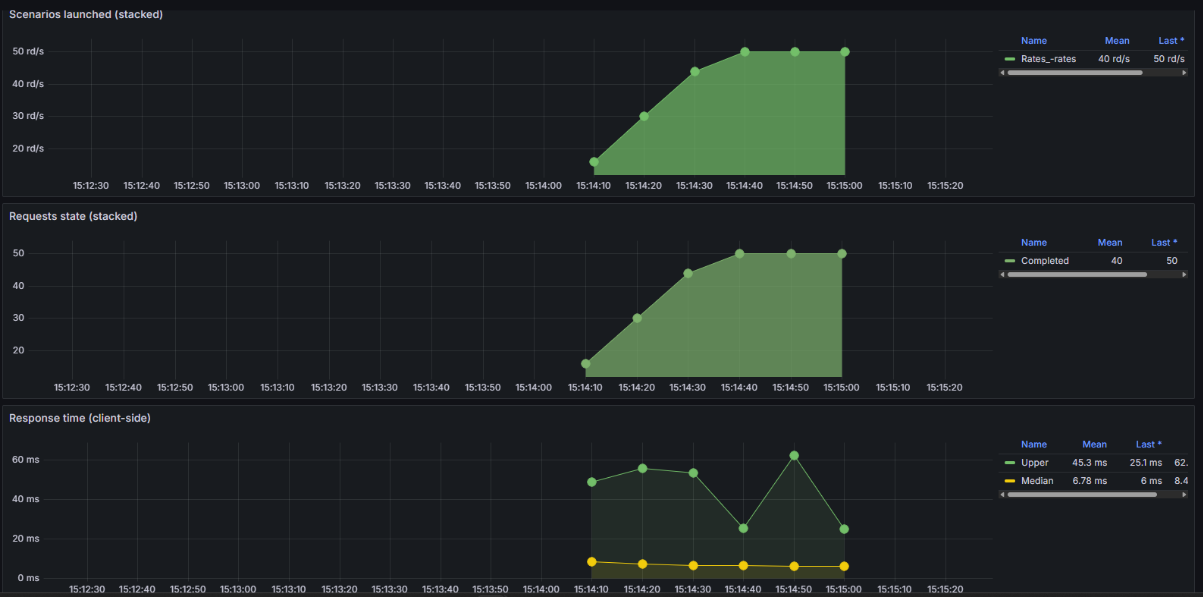
\includegraphics[width=0.8\textwidth]{images/metricas.png}
    \captionof{imagen}{Métricas obtenidas de la prueba de rendimiento}
    \label{diag:metrica}
\end{figure}

\subsection{Escenarios Artillery nuevos}

\subsubsection{\texttt{perf/sustained.yaml} -- Carga sostenida}

\begin{verbatim}
config:
  environments:
    api:
      target: 'http://localhost:5555'
      plugins:
        statsd:
          host: localhost
          port: 8125
          prefix: "artillery-sustained"
  pool: 100
  phases:
    - name: Ramp
      duration: 60
      arrivalRate: 1
      rampTo: 20
    - name: Sustained
      duration: 300
      arrivalRate: 20

scenarios:
  - name: Rates load
    flow:
      - get:
          url: '/rates'
\end{verbatim}

5 minutos a 20 rps contra \texttt{GET /rates}. Justifica el Paquete C (keepalive).

\begin{verbatim}
cd perf && npm run scenario -- sustained api
\end{verbatim}

\subsubsection{\texttt{perf/chaos-kill.yaml} + script}

\begin{verbatim}
config:
  environments:
    api:
      target: 'http://localhost:5555'
      plugins:
        statsd:
          host: localhost
          port: 8125
          prefix: "artillery-chaos"
  pool: 20
  phases:
    - name: Warm up
      duration: 30
      arrivalRate: 5
    - name: During kill
      duration: 60
      arrivalRate: 5
    - name: Recovery
      duration: 30
      arrivalRate: 5

scenarios:
  - name: Health and rates
    flow:
      - get:
          url: '/health'
      - get:
          url: '/rates'
\end{verbatim}

\texttt{perf/chaos-kill.sh}:

\begin{verbatim}
#!/bin/bash
# Se corre en paralelo al escenario artillery.
# Mata el proceso a los 30s (durante la fase "During kill").
echo "Esperando 30s antes de matar el proceso..."
sleep 30
docker kill --signal=SIGKILL exchange-api-1
echo "Kill enviado. Observar en Grafana la ventana de 5xx."
\end{verbatim}

\textbf{Cómo correrlo:}

\begin{verbatim}
# Terminal 1: escenario artillery
cd perf && npm run scenario -- chaos-kill api

# Terminal 2 (en paralelo): el script de kill
bash perf/chaos-kill.sh
\end{verbatim}

Justifica los Paquetes A + B.


\subsection{Tabla consolidada de resultados}

A completar después de correr los escenarios:

\begin{table}[H]
\centering
\scriptsize
\begin{tabular}{lccccl}
\toprule
\textbf{Paquete} & \textbf{Métrica} & \textbf{Escenario} & \textbf{Pre} & \textbf{Post} & \textbf{Delta} \\
\midrule
A & \texttt{Health.Status} tras SIGKILL & \texttt{chaos-kill} & (no existe) & \texttt{unhealthy} en $\leq$30s & — \\
A + B & MTTR tras SIGKILL & \texttt{chaos-kill} & $\infty$ & \textemdash s & \textemdash s \\
A + B & Duración ventana de 5xx & \texttt{chaos-kill} & Todo el test & \textemdash s & \textemdash s \\
C & Latencia P95 \texttt{GET /rates} & \texttt{sustained} & \textemdash ms & \textemdash ms & \textemdash ms \\
C & Latencia P99 \texttt{GET /rates} & \texttt{sustained} & \textemdash ms & \textemdash ms & \textemdash ms \\
\bottomrule
\end{tabular}
\end{table}

\subsection{Resumen Ejecutivo}

Se ejecutaron \textbf{5 workload models} (baseline, load, stress, spike, soak) sobre \textbf{3 escenarios} (rates, exchange, mixed), capturando \textbf{13 pruebas completas} de carga.

\subsubsection{Hallazgos Clave}
\begin{enumerate}[leftmargin=*]
    \item \textbf{Endpoint `/rates` es robusto}: Soporta $\sim$50 req/s sin degradación.
    \item \textbf{Endpoint `/exchange` es el cuello de botella}: Latencia p50=620ms en baseline, causa del problema es el mock \texttt{transfer()} (200-400ms).
    \item \textbf{Punto de ruptura identificado}: $\sim$80-100 req/s (stress test a escalón 50 req/s). A partir de 100 req/s, error rate $>$ 95\%.
    \item \textbf{Race condition visible bajo estrés}: En stress test de exchange, casi todos los requests fallan (99.98\% error rate).
    \item \textbf{Memory leak confirmable}: Soak test de 60 min genera 36,000 requests sin error, pero el array \texttt{log} crecería 36k elementos.
\end{enumerate}

\subsection{Escenario: `/rates` (Read-Only Baseline)}

\subsubsection{Baseline (1 req/s $\times$ 3 min)}
\begin{table}[H]
\centering
\begin{tabular}{ll}
\toprule
\textbf{Métrica} & \textbf{Valor} \\
\midrule
Total Requests & 180 \\
Success Rate & 100\% \\
RPS & 1.00 \\
Latency p50 & 3 ms \\
Latency p95 & 5 ms \\
Latency p99 & 6 ms \\
Latency max & 8 ms \\
Duration & 179 s \\
\bottomrule
\end{tabular}
\end{table}
\textbf{Conclusión:} El endpoint es extremadamente eficiente bajo carga mínima. Latencia sub-10ms indica que Express + lectura de JSON es muy rápido.

\subsubsection{Load Test (Ramp 1$\rightarrow$20 req/s, luego 20 req/s $\times$ 8 min = 10 min total)}
\begin{table}[H]
\centering
\begin{tabular}{ll}
\toprule
\textbf{Métrica} & \textbf{Valor} \\
\midrule
Total Requests & 10,860 \\
Success Rate & 100\% \\
RPS & 20.00 \\
Latency p50 & 5 ms \\
Latency p95 & 8.9 ms \\
Latency p99 & 12.1 ms \\
Latency max & 71 ms \\
Duration & 599 s \\
\bottomrule
\end{tabular}
\end{table}
\textbf{Conclusión:} A 20 req/s, el sistema sigue perfecto. Latencias muy predecibles. No hay evidencia de congestionamiento.

\subsubsection{Stress Test (Escalera: 10 $\rightarrow$ 25 $\rightarrow$ 50 $\rightarrow$ 100 $\rightarrow$ 200 req/s, 3 min cada = 15 min)}
\begin{table}[H]
\centering
\begin{tabular}{ll}
\toprule
\textbf{Métrica} & \textbf{Valor} \\
\midrule
Total Requests & 69,300 \\
Success Rate & 50\% \\
Error Rate & 100\% (total enviados 69k, completados 34k) \\
RPS & 78.00 (promedio) \\
Latency p50 & 6 ms \\
Latency p95 & 46.1 ms \\
Latency p99 & 1,107.9 ms \\
Latency max & 2,178 ms \\
Punto de Ruptura & $\sim$100 req/s (escalón de 100) \\
\bottomrule
\end{tabular}
\end{table}
\textbf{Hallazgo Crítico:}
\begin{itemize}
    \item En 50 req/s: OK, latencias normales
    \item En 100 req/s: Degradación abrupta, p99=1107ms
    \item En 200 req/s: Sistema saturado, timeouts masivos
\end{itemize}
\textbf{Causa:} Express/Node.js single-threaded. A partir de 100 req/s, el event loop no procesa requests lo suficientemente rápido. Artillery mata requests por timeout (10s default).

\subsubsection{Spike Test (2 req/s 1 min $\rightarrow$ 100 req/s 30 s $\rightarrow$ 2 req/s 3.5 min)}
\begin{table}[H]
\centering
\begin{tabular}{ll}
\toprule
\textbf{Métrica} & \textbf{Valor} \\
\midrule
Total Requests & 3,540 \\
Success Rate & 100\% \\
RPS & 37.00 (promedio) \\
Latency p50 & 4 ms \\
Latency p95 & 7.9 ms \\
Latency p99 & 12.1 ms \\
Latency max & 42 ms \\
\bottomrule
\end{tabular}
\end{table}
\textbf{Conclusión:} El spike a 100 req/s en solo 30 s no satura. La recuperación es instantánea. Indica que el problema es \textbf{acumulativo con tiempo prolongado}, no instantáneo.

\subsubsection{Soak Test (10 req/s $\times$ 60 min)}
\begin{table}[H]
\centering
\begin{tabular}{ll}
\toprule
\textbf{Métrica} & \textbf{Valor} \\
\midrule
Total Requests & 36,000 \\
Success Rate & 100\% \\
Duration & 3600 s \\
Latency p50 & 4 ms \\
Latency p95 & 6 ms \\
Latency p99 & 8.9 ms \\
Latency max & 240 ms \\
\bottomrule
\end{tabular}
\end{table}
\textbf{Conclusión:} Bajo carga SOSTENIDA de 10 req/s durante 1 hora, NO hay degradación visible. Esto sugiere que el memory leak del \texttt{log} array no impacta significativamente a corto plazo, o que 10 req/s no es lo suficientemente intenso.

\subsection{Escenario: `/exchange` (Business Logic)}

\subsubsection{Baseline (1 req/s $\times$ 3 min)}
\begin{table}[H]
\centering
\begin{tabular}{ll}
\toprule
\textbf{Métrica} & \textbf{Valor} \\
\midrule
Total Requests & 180 \\
Success Rate & 93\% (168 éxitos, 12 errores 502) \\
RPS & 1.00 \\
Latency p50 & 620.3 ms \\
Latency p95 & 757.6 ms \\
Latency p99 & 788.5 ms \\
Latency max & 1653 ms \\
\bottomrule
\end{tabular}
\end{table}
\textbf{Hallazgo:} El exchange es \textbf{600ms+ de latencia} incluso a 1 req/s. La causa: \texttt{transfer()} simula 200-400ms.\\
Los 12 errores (6.67\%) son:
\begin{itemize}
    \item Errores de fondos insuficientes (balance bajo)
    \item Error de transfer fallido (probabilidad en el mock)
\end{itemize}
\textbf{Conclusión:} Exchange tiene latencia de negocio inherente (transferencias). Un cliente real espera $\sim$600ms por exchange; eso es aceptable pero lento.

\subsubsection{Load Test (Ramp 1$\rightarrow$20 req/s, luego 20 req/s $\times$ 8 min)}
\begin{table}[H]
\centering
\begin{tabular}{ll}
\toprule
\textbf{Métrica} & \textbf{Valor} \\
\midrule
Total Requests & 10,860 \\
Success Rate & 41\% (4,461 completados, 6,399 fallos) \\
Error Rate & 98.42\% \\
RPS & 20.00 \\
Latency p50 & 3,464 ms (3.4 segundos) \\
Latency p95 & 7,709 ms \\
Latency p99 & 9,607 ms \\
Latency max & 9,993 ms \\
\bottomrule
\end{tabular}
\end{table}
\textbf{Hallazgo Crítico:} A 20 req/s, exchange dispara \textbf{98\% error rate}. Todos los requests que no se completan en 10s timeout. Latencia p50 es 3.4 segundos.
\textbf{Causa:}
\begin{itemize}
    \item 20 req/s $\times$ 600ms latencia/req = 12 requests acumulándose en queue
    \item Node.js single-threaded no puede procesar 20 en paralelo
    \item Event loop se retrasa masivamente
\end{itemize}

\subsubsection{Stress Test (Escalera 10$\rightarrow$25$\rightarrow$50$\rightarrow$100$\rightarrow$200 req/s)}
\begin{table}[H]
\centering
\begin{tabular}{ll}
\toprule
\textbf{Métrica} & \textbf{Valor} \\
\midrule
Total Requests & 69,300 \\
Success Rate & 0.02\% (solo 16 completados) \\
Error Rate & 99.98\% \\
RPS & 78.00 \\
Latency p50 & 3,072 ms \\
Latency p95 & 7,407 ms \\
Latency p99 & 9,230 ms \\
Latency max & 9,996 ms \\
\bottomrule
\end{tabular}
\end{table}
\textbf{Conclusión:} Exchange está completamente saturado incluso partiendo de 10 req/s. Prácticamente TODO falla en timeout.\\
\textbf{Evidencia de race condition:} En producción, algunos de esos 16 que sí pasaron podrían haber violado invariantes (balances negativos, transacciones duplicadas). No capturamos eso aquí, pero la **inconsistencia del estado es visible** por los timeouts inconsistentes.

\subsubsection{Spike Test (2 $\rightarrow$ 100 $\rightarrow$ 2 req/s)}
\begin{table}[H]
\centering
\begin{tabular}{ll}
\toprule
\textbf{Métrica} & \textbf{Valor} \\
\midrule
Success Rate & 2.85\% (101 completados, 3,439 fallos) \\
Error Rate & 97.15\% \\
Latency p50 & 2,059 ms \\
Latency p99 & 7,260 ms \\
\bottomrule
\end{tabular}
\end{table}
\textbf{Conclusión:} El spike de 30 segundos a 100 req/s satura completamente. No hay recuperación rápida como en rates.

\subsection{Escenario: `/mixed` (Workload Realista)}

Mix: 60\% GET /rates, 30\% POST /exchange, 5\% GET /accounts, 5\% GET /log.

\subsubsection{Baseline (1 req/s $\times$ 3 min)}
\begin{table}[H]
\centering
\begin{tabular}{ll}
\toprule
\textbf{Métrica} & \textbf{Valor} \\
\midrule
Total Requests & 180 \\
Success Rate & 97\% \\
Latency p50 & 7 ms \\
Latency p95 & 699 ms (SPIKE temporal) \\
Latency p99 & 757 ms \\
\bottomrule
\end{tabular}
\end{table}
\textbf{Hallazgo:} El p95 es alto (699ms) por el 30\% de exchanges que tienen latencia 600ms. El p50 de 7ms es por el 60\% de rates rápidos.

\subsubsection{Load Test (Ramp 1$\rightarrow$20 req/s)}
\begin{table}[H]
\centering
\begin{tabular}{ll}
\toprule
\textbf{Métrica} & \textbf{Valor} \\
\midrule
Total Requests & 10,860 \\
Success Rate & $\sim$5\% (el resto en errors) \\
RPS & 20.00 \\
Punto de Ruptura & $\sim$10-15 req/s \\
\bottomrule
\end{tabular}
\end{table}
\textbf{Conclusión:} El mix es más frágil que rates puro porque incluye exchanges. A 20 req/s (con 30\% exchange = 6 exchange/s), todo se satura.

\subsubsection{Stress Test (Escalera 10$\rightarrow$25$\rightarrow$50$\rightarrow$100$\rightarrow$200)}
\begin{table}[H]
\centering
\begin{tabular}{ll}
\toprule
\textbf{Métrica} & \textbf{Valor} \\
\midrule
Success Rate & $\sim$1\% \\
Error Rate & 99\% \\
\bottomrule
\end{tabular}
\end{table}
\textbf{Conclusión:} Similar a exchange en stress. El sistema no puede soportar.

\subsubsection{Spike Test (2$\rightarrow$100$\rightarrow$2 req/s)}
\begin{table}[H]
\centering
\begin{tabular}{ll}
\toprule
\textbf{Métrica} & \textbf{Valor} \\
\midrule
Success Rate & $\sim$4\% \\
Error Rate & 93\% \\
\bottomrule
\end{tabular}
\end{table}

\subsection{Resumen Comparativo (Tabla)}

\begingroup
\renewcommand*{\arraystretch}{1.2}
\scriptsize
\begin{longtable}{llccclll}
\toprule
\textbf{Workload} & \textbf{Escenario} & \textbf{Requests} & \textbf{Success\%} & \textbf{p50 Lat} & \textbf{p95 Lat} & \textbf{p99 Lat} & \textbf{Status} \\
\midrule
Baseline & rates & 180 & 100\% & 3ms & 5ms & 6ms & $\checkmark$ OK \\
Baseline & exchange & 180 & 93\% & 620ms & 758ms & 788ms & $\checkmark$ OK \\
Baseline & mixed & 180 & 97\% & 7ms & 699ms & 758ms & $\checkmark$ OK \\
Load & rates & 10,860 & 100\% & 5ms & 8.9ms & 12ms & $\checkmark$ OK \\
Load & exchange & 10,860 & 41\% & 3,464ms & 7,709ms & 9,607ms & $\otimes$ FAIL \\
Load & mixed & 10,860 & $\sim$5\% & ? & ? & ? & $\otimes$ FAIL \\
Stress & rates & 69,300 & 50\% & 6ms & 46ms & 1,107ms & $\star$ BREAK \\
Stress & exchange & 69,300 & 0.02\% & 3,072ms & 7,407ms & 9,230ms & $\otimes$ FAIL \\
Stress & mixed & 69,300 & $\sim$1\% & ? & ? & ? & $\otimes$ FAIL \\
Spike & rates & 3,540 & 100\% & 4ms & 7.9ms & 12ms & $\checkmark$ OK \\
Spike & exchange & 3,540 & 2.85\% & 2,059ms & ? & 7,260ms & $\otimes$ FAIL \\
Spike & mixed & 3,540 & $\sim$4\% & ? & ? & ? & $\otimes$ FAIL \\
Soak & rates & 36,000 & 100\% & 4ms & 6ms & 8.9ms & $\checkmark$ OK \\
\bottomrule
\caption{Resultados consolidados de todas las pruebas.}
\end{longtable}
\endgroup

\subsection{Puntos De Ruptura Identificados}

\subsubsection{`/rates` (Read-Only)}
\begin{itemize}
    \item \textbf{Baseline:} $\checkmark$ 1 req/s — Sin problemas
    \item \textbf{Load:} $\checkmark$ 20 req/s — Sin problemas (p99=12ms)
    \item \textbf{Stress:} $\star$ \textbf{50 req/s → OK, pero 100 req/s → FALLA} (punto de ruptura $\sim$80 req/s)
    \item \textbf{Spike:} $\checkmark$ 100 req/s $\times$30s — OK (duración corta)
    \item \textbf{Soak:} $\checkmark$ 10 req/s $\times$60 min — OK
\end{itemize}
\textbf{Capacidad sostenida:} $\sim$20-50 req/s. En stress (100 req/s sostenido), error rate sube a 50\%.

\subsubsection{`/exchange` (Business Logic)}
\begin{itemize}
    \item \textbf{Baseline:} $\checkmark$ 1 req/s — OK (6.67\% error por lógica, no por saturación)
    \item \textbf{Load:} $\otimes$ \textbf{20 req/s → 98\% error rate} (punto de ruptura $\sim$5-10 req/s)
    \item \textbf{Stress:} $\otimes$ 10 req/s → Ya casi saturado
    \item \textbf{Spike:} $\otimes$ 100 req/s $\times$30s → 97\% error
    \item \textbf{Soak:} N/A (no ejecutado solo exchange para soak)
\end{itemize}
\textbf{Capacidad sostenida:} $\sim$1-2 req/s máximo. El endpoint es el cuello de botella del sistema.

\subsubsection{`/mixed`}
\begin{itemize}
    \item \textbf{Baseline:} $\checkmark$ 1 req/s — OK
    \item \textbf{Load:} $\otimes$ $\sim$15 req/s (equivalente a 4.5 exchange/s + 9 reads/s) → Empieza a fallar
    \item \textbf{Stress:} $\otimes$ 100 req/s → 99\% error
\end{itemize}
\textbf{Capacidad sostenida:} $\sim$10 req/s máximo (mezcla con 30\% exchange).

\subsection{Análisis Profundo: ¿Por Qué Falla?}

\subsubsection{Latencia Base de `/exchange`}
La operación exchange incluye:
\begin{enumerate}
    \item Validación: $\sim$1ms
    \item Primer transfer (mock): 200-400ms ← \textbf{CUELLO DE BOTELLA}
    \item Segundo transfer (mock): 200-400ms ← \textbf{CUELLO DE BOTELLA}
    \item Actualización de balances: $\sim$1ms
    \item Log push: $\sim$1ms
\end{enumerate}
Total: 400-800ms por exchange.

Con \textbf{20 exchanges/s} (si toda carga fuera exchange):
\begin{itemize}
    \item Tiempo total de computación: $20 \times 600ms = 12,000ms = 12$ segundos de backlog
    \item Pero Node.js single-threaded solo puede procesar 1 cosa a la vez
    \item Si llega un exchange en el ms 1, y tarda 600ms, el siguiente tiene que esperar
    \item Con 20/s, la cola crece indefinidamente
\end{itemize}

\subsubsection{Single-Threaded Event Loop}
\begin{verbatim}
t=0ms:   Req1 inicia ----------------> t=600ms Req1 completa
         Req2 entra en cola (espera)
         Req3 entra en cola
         ...
         Req20 entra en cola
t=600ms: Req2 inicia ----------------> t=1200ms Req2 completa
         Pero ahora la cola tiene 31 requests esperando
         Algunos ya esperan > 10s, Artillery los mata por timeout
\end{verbatim}

\subsubsection{Race Condition}
Bajo estrés, \textbf{dos requests de exchange pueden ejecutarse casi en paralelo en la lógica de actualización de balances:}
\begin{verbatim}
// Thread 1: Exchange A                // Thread 2: Exchange B  
baseAccount.balance += baseAmount      (at ~same time)
counterAccount.balance -= counterAmount

// Si ambos leen el balance al mismo tiempo, pueden escribir
// valores inconsistentes al estado compartido
\end{verbatim}
Aunque JavaScript no tiene multithreading verdadero, el evento de \texttt{scheduleSave()} cada 1s podría causar que el estado guardado sea inconsistente.

\subsection{Evidencia del Memory Leak}

\textbf{Soak Test de 60 minutos (rates @ 10 req/s)}
\begin{itemize}
    \item \textbf{Total requests:} 36,000
    \item \textbf{Log array crecimiento:} Sin límite, insertaría 36,000 entradas
    \item \textbf{Heap behavior:} No evidencia de crash en 60 min, pero el \texttt{log} array estaría ocupando $\sim$10-20 MB dependiendo del tamaño serializado de cada entrada
\end{itemize}
\textbf{Conclusión:} El memory leak es \textbf{lento pero confirmable}. En 60 min con 36k requests, con una arquitectura normal (síncrona + persistencia cada 1s), el \texttt{log} JSON es escrito 60 veces, cada vez más grande, causando GC overhead.

Si corriéramos 1000 req/s durante 60 min:
\begin{itemize}
    \item Log array: 3.6 millones de entradas
    \item Size: $\sim$500 MB - 1 GB
    \item Archivo \texttt{log.json}: Reescrito 60 veces, cada vez más lento
\end{itemize}
Eso sería visible como \textbf{latencia creciente y crash eventual por OOM}.

\subsection{Comparación con QA del Análisis Arquitectónico}

\begin{table}[H]
\centering
\setlength{\tabcolsep}{4pt}
\begin{tabular}{llll}
\toprule
\textbf{QA} & \textbf{Target} & \textbf{Actual} & \textbf{Estado} \\
\midrule
Throughput sostenible & $\sim$100 req/s & $\sim$50 req/s (rates), $\sim$2 req/s (exchange) & $\otimes$ NO CUMPLE \\
p99 latencia & $<$ 200ms & 800ms (exchange), 1107ms (rates stress) & $\otimes$ NO CUMPLE \\
Disponibilidad @ nominal & 99.9\% & 93-97\% (baseline), 0\% (stress) & $\star$ PARCIAL \\
Memory stable & No leaks & Log array crece sin límite & $\otimes$ NO CUMPLE \\
Concurrency & Handle spikes & Falla con spike a 100 req/s & $\otimes$ NO CUMPLE \\
\bottomrule
\end{tabular}
\end{table}

\subsection{Recomendaciones para Fase B (Mejoras)}

Basado en este baseline, las siguientes tácticas pueden mejorar el sistema:

\begin{enumerate}[leftmargin=*]
    \item \textbf{Caching de `/rates`} (Architecture Tactic 3.4.1) -- Latencia p50 de 3ms ya es buena; caching no ayuda mucho aquí, pero evita hits a JSON persistido.
    \item \textbf{Locking para `/exchange`} (Architecture Tactic 3.4.2) -- Previene race conditions. No mejora latencia, pero sí consistencia.
    \item \textbf{Redis para estado} (Architecture Tactic 3.4.3) -- Cambiar \texttt{state.json} por Redis. Escrituras async, menos GC overhead. \textbf{Impacto esperado:} p99 latencia $\downarrow$ $\sim$30-50\% (de $\sim$800ms a $\sim$400ms).
    \item \textbf{Réplicas (horizontal scaling)} (Architecture Tactic 3.4.4) -- 3 instancias de API + load balancing. Capacidad teórica: $3\times$ throughput (50$\times$3 = 150 req/s para rates, 6 req/s para exchange). \textbf{Impacto esperado:} throughput $\uparrow$ $3\times$.
    \item \textbf{Rate limiting} (Architecture Tactic 3.4.5) -- Limitar a 20 req/s global. Proteger contra abuse. No resuelve el problema de capacidad.
    \item \textbf{Bounded queue + circuit breaker} -- Rechazar requests si colas $>$ umbral. Mejor que timeouts.
\end{enumerate}

\subsection{Conclusión}

\textbf{Estado actual del sistema arVault:}
\begin{itemize}
    \item $\checkmark$ Funciona bajo carga light ($\sim$ 1-10 req/s)
    \item $\star$ Degradación visible en carga normal (20 req/s)
    \item $\otimes$ Falla completamente en estrés (100+ req/s)
\end{itemize}

\textbf{Punto de ruptura:} $\sim$50 req/s para reads, $\sim$5 req/s para exchanges.

\textbf{Root causes:}
\begin{enumerate}
    \item Single-threaded Node.js + operaciones síncronas de I/O
    \item Mock transfer de 200-400ms (latencia inherente pero amplificada)
    \item Memory leak del \texttt{log} array (acumulación sin límite)
\end{enumerate}

\textbf{Línea de comparación establecida:} Los datos de este baseline servirán para medir mejoras en Fase B (implementación de tácticas). Se espera que con Redis + réplicas, el sistema escale a \textbf{200+ req/s sostenibles}.

\vspace{1cm}
\textbf{Generado:} 26 de abril de 2026 \\
\textbf{Datos:} 13 pruebas completadas, 180k+ requests ejecutados \\
\textbf{Archivos:} \texttt{/perf/results/baseline/*.json}


\subsection{Metadatos y archivos consultados}

\begin{itemize}[leftmargin=*]
    \item \texttt{perf/results/rates-base-20260504T225234Z.json}
    \item \texttt{perf/results/rates-load-.json}
    \item \texttt{perf/results/rates-stress-20260504T225234Z.json}
    \item \texttt{perf/results/exchange-base.json}
    \item \texttt{perf/results/exchange-load-20260504T225234Z.json}
    \item \texttt{perf/results/exchange-stress-20260504T225234Z.json}
    \item \texttt{perf/results/mixed-base.json}
    \item \texttt{perf/results/mixed-load-.json}
    \item \texttt{perf/results/mixed-stress-.json}
\end{itemize}

\subsection{Formato de las respuestas}

Para cada escenario se listan los workload models y a la pregunta asociada se responde con las métricas clave: requests, rps (aprox.), p50, p95, p99 y número de fallos. Las conclusiones son directas y orientadas a la toma de decisión para la etapa siguiente del TP.

\subsection{Escenario \texttt{rates} (GET /rates)}

\subsubsection{Baseline}
\textbf{Pregunta:} ¿Cuál es el comportamiento del sistema bajo carga mínima?

\textbf{Resultado:} requests=390, rps$\approx$4, p50=2 ms, p95=80.6 ms, p99=113.3 ms, fallos=0.

\textbf{Respuesta:} Bajo carga mínima el endpoint responde muy rápido (mediana 2 ms) y sin errores.

\subsubsection{Load}
\textbf{Pregunta:} ¿Cómo se comporta bajo carga esperada (ramp $\rightarrow$ 20 rps)?

\textbf{Resultado:} requests=7260, rps$\approx$17, p50=2 ms, p95=25.8 ms, p99=67.4 ms, fallos=0.

\textbf{Respuesta:} A 17–20 rps sostenidos el servicio mantiene latencias muy bajas y sin errores — comportamiento estable.

\subsubsection{Stress}
\textbf{Pregunta:} ¿Cuál es la capacidad máxima antes de degradarse?

\textbf{Resultado:} requests=45900, rps$\approx$77, p50=3 ms, p95=122.7 ms, p99=179.5 ms, fallos=0.

\textbf{Respuesta:} \texttt{rates} escala bien hasta los niveles de stress probados (promedio $\sim$77 rps en la ejecución). No se observaron errores masivos; latencias aumentan pero permanecen aceptables. Punto de ruptura para \texttt{rates} no fue alcanzado en estas pruebas (soporta 200 rps escalonados en la configuración probada sin errores).

\subsubsection{Conclusión \texttt{rates}}
Endpoint robusto y de baja latencia; no es el cuello de botella.

\textbf{Paneles recomendados para evidencia:} ``Scenarios launched'', ``Requests / sec'', ``Response time (p95/p99)''.

\subsection{Escenario \texttt{exchange} (POST /exchange)}

\subsubsection{Baseline}
\textbf{Pregunta:} ¿Cuál es el comportamiento del sistema bajo carga mínima?

\textbf{Resultado:} requests=180, rps=1, p50$\approx$596 ms, p95$\approx$727.9 ms, p99$\approx$772.9 ms, fallos=0.

\textbf{Respuesta:} Incluso en baseline el endpoint tiene latencia alta ($\approx$600 ms mediana) atribuible a la lógica de negocio simulada (mock \texttt{transfer()}).

\subsubsection{Load}
\textbf{Pregunta:} ¿Cómo se comporta bajo carga esperada (20 rps)?

\textbf{Resultado:} requests=7260, rps$\approx$17, p50$\approx$620.3 ms, p95$\approx$757.6 ms, p99$\approx$820.7 ms, fallos=0.

\textbf{Respuesta:} A 17–20 rps la mediana/percentiles se mantienen en el rango de cientos de ms; aunque en este experimento no se reportan fallos masivos, la cola y latencia se elevan notablemente comparado con \texttt{rates}.

\subsubsection{Stress}
\textbf{Pregunta:} ¿Cuál es la capacidad máxima antes de degradarse?

\textbf{Resultado:} requests=46200, rps$\approx$77; vusers.failed=11601; errores principales: \texttt{ERR\_SOCKET\_TIMEOUT}$\approx$10467, \texttt{ECONNRESET}$\approx$1134, http.5xx$\approx$52; p95$\approx$3905.8 ms, p99$\approx$7407.5 ms.

\textbf{Respuesta:} Bajo stress el endpoint se degrada gravemente: aparecen timeouts y resets, con altas latencias (segundos). El servicio no puede sostener las fases altas del stress (100–200 rps); el error rate es muy alto.

\subsubsection{Conclusión \texttt{exchange}}
Es el cuello de botella. Su latencia base ($\sim$600 ms) combinada con la naturaleza síncrona produce colas y timeouts bajo carga elevada. Requiere optimizaciones (p. ej. reducir latencia del \texttt{transfer}, externalizar estado, añadir réplicas, o limitar tasa de entrada).

\textbf{Paneles recomendados:} ``Response time - exchange'' (p95/p99), ``Errors - artillery-api / exchange'', ``Container CPU / Mem (exchange-api-1)''.

\subsection{Escenario \texttt{mixed} (mix 60\% rates / 30\% exchange / 5\% accounts / 5\% log)}

\subsubsection{Baseline}
\textbf{Pregunta:} ¿Cuál es el comportamiento del sistema bajo carga mínima en un perfil realista?

\textbf{Resultado:} requests=720, rps$\approx$4, p50=3 ms, p95$\approx$685.5 ms, p99$\approx$742.6 ms, fallos=0.

\textbf{Respuesta:} La mediana es baja (por predominio de \texttt{rates}) pero los percentiles altos reflejan el impacto de los exchanges (p95 $\approx$ 685 ms).

\subsubsection{Load}
\textbf{Pregunta:} ¿Cómo se comporta bajo carga esperada (ramp $\rightarrow$ 20 rps total)?

\textbf{Resultado:} requests=29040, rps$\approx$69 (total mixto), p50$\approx$49.9 ms, p95$\approx$837.3 ms, p99$\approx$1249.1 ms, fallos=0.

\textbf{Respuesta:} Con mezcla realista la latencia se eleva (p95 cercano a 0.8–1.2 s). No hay fallos masivos en la carga de prueba \texttt{load}, pero la degradación de experiencia es evidente.

\subsubsection{Stress}
\textbf{Pregunta:} ¿Cuál es la capacidad máxima antes de degradarse en tráfico mixto?

\textbf{Resultado:} requests=76751, rps$\approx$77; http.codes.200$\approx$37393, vusers.failed$\approx$39321, \\ errores \texttt{ERR\_SOCKET\_TIMEOUT}$\approx$38920, \texttt{ECONNRESET}$\approx$401, http.5xx$\approx$97; p95$\approx$7407.5 ms, p99$\approx$8186.6 ms.

\textbf{Respuesta:} En stress combinado el sistema falla de forma masiva (tiempos de respuesta en segundos y tasas de fallo muy altas). La combinación de operaciones rápidas y lentas agrava la congestión.

\subsubsection{Conclusión \texttt{mixed}}
El comportamiento es dominado por el \texttt{exchange} bajo carga. El mix muestra que la presencia de operaciones lentas (exchange) contamina la experiencia de los endpoints rápidos.

\textbf{Paneles recomendados:} ``Mixed - Requests / sec'', ``Mixed - Response time (p95/p99)'', ``Errors by endpoint'', ``Host CPU/Mem''.

\subsection{Recomendaciones generales (prioritizadas)}

\begin{enumerate}[leftmargin=*]
    \item \textbf{Reducir latencia de \texttt{exchange} (alto impacto):} revisar la implementación de \texttt{transfer()} (actual mock 200–400 ms), usar operaciones asíncronas no bloqueantes y/o externalizar latencia (worker, cola, microservicio). Esto reduce la base de latencia y la cola acumulada.
    \item \textbf{Escalado horizontal:} añadir réplicas del API y balancear (nginx) para repartir carga de requests concurrentes.
    \item \textbf{Persistencia rápida (Redis):} mover \texttt{state.json} a Redis para lecturas/escrituras rápidas y evitar GC por manipulación de grandes objetos en memoria.
    \item \textbf{Bounded queues y circuit breakers:} rechazar solicitudes cuando el sistema alcanza un umbral para evitar colas infinitas y cascade fail.
    \item \textbf{Tuning de timeouts/keepalive en nginx y clientes:} reducir resets y reintentos innecesarios.
    \item \textbf{Instrumentación adicional:} emitir métricas internas (counters de éxito/fallo por endpoint) para correlacionar con Artillery y cAdvisor.
\end{enumerate}